% !TEX program = xelatex
\documentclass[UTF8,zihao=-4,fontset=none,oneside]{ctexrep}
\newcommand{\worktitle}{RISC-V 边缘AI加速系统}
\newcommand{\workshorttitle}{TriHaRiscv v3 技术文档}
\newif\ifreportdraft
\reportdrafttrue
\newif\ifreleaseappendix
\releaseappendixfalse

\usepackage{triha-report}
\begin{document}
\pagenumbering{Roman}
\chapter*{\worktitle}
\addcontentsline{toc}{chapter}{摘\ \ 要}

\begin{center}
\sffamily\bfseries\zihao{-2} 摘\ \ 要
\end{center}

\begingroup
\setlength{\parskip}{0pt}
\linespread{1.0}\selectfont
\tableofcontents
\endgroup
\clearpage
\pagenumbering{arabic}
\chapter{作品概述}

\section{功能与特性}

TriHaRiscv\footnote{TriHaRiscv的命名灵感来源于团队名称“哈哈哈”（即Triple Ha）。}是基于自研RISC-V CPU与NPU的异构视觉处理系统。
设计以CPU实现、国产FPGA集成及性能分析为主线，通过人脸检测和预设人物头像叠加展示处理器、计算加速和视频处理的协同工作。
系统在盘古100pro+平台上集成CPU、NPU、AXI互连、存储及HDMI视频链路，具备以下功能与特性：
\begin{itemize}
    \item CPU采用六级流水线、单发射、顺序执行与顺序提交结构，支持RV32IM指令集、CSR访问及\texttt{FENCE.I}指令。
    \item CPU运行于机器模式，支持异常处理、中断响应与返回，提供周期计数；仿真通过WB提交观测与流水线事件分析执行效率。
    \item I-Cache与D-Cache各为16\,KiB，采用两路组相联、32\,B缓存行；D-Cache采用写回、写分配策略，支持缓存行清理与失效。
    \item 动态分支预测采用512项两位计数器BHT、512项直接映射BTB和4项返回地址栈；64\,bit取指包与两项取指FIFO为单发射流水线供给指令。
    \item NPU采用INT8乘法、INT32累加，提供64和128乘加通路配置，支持普通卷积、逐点卷积、深度卷积及网络所需辅助算子。
    \item CPU按算子配置NPU，NPU在内部完成分块循环；DMA搬运权重、特征图和计算结果，完成通知与输出写响应保持一致。
    \item 采用32\,bit AXI4-Lite控制接口和128\,bit AXI4数据DMA接口，通过桥接连接CPU访存接口与DDR控制器。
    \item 集成Boot ROM、片上SRAM及1\,GB板载DDR3，划分CPU私有可缓存区和DMA不可缓存共享区。
    \item 集成UART、GPIO、定时器、SPI、I\textsuperscript{2}C和外部中断控制，支持程序装载、板级初始化及运行状态记录。
    \item HDMI输入与输出均为800$\times$600、标称60\,Hz，检测覆盖完整输入画面，显示端按帧切换RAW、BOX和AVATAR全屏模式。
    \item 视频硬件生成400$\times$300 RGB888预览图和320$\times$320 UINT8 BGR NCHW输入，完成双线性缩放、补边、行缓冲、头像映射及Alpha混合，CPU提交帧地址及显示参数。
    \item 裸机运行YuNet人脸检测，CPU完成定点解码、NMS和主人脸选择，三帧槽管理采集、处理和显示的数据生命周期。
\end{itemize}

\section{应用领域}

系统面向交互式视觉终端、数字镜面和嵌入式视觉等场景。输入视频经YuNet检测后，显示端在完整原图上叠加人脸框、关键点或主人脸对应的预设动漫头像。
用户通过MODE按键切换原图、检测标记和头像叠加三种全屏模式，切换在有效图像起点生效。
主人脸按有效框面积、置信度及固定候选顺序选择，头像由软件配置，叠加采用二维缩放、平移与透明混合。

模型准备和素材转换在主机离线完成。程序、权重和素材装载后，FPGA独立执行图像处理、网络推理、检测后处理和视频输出。
同一硬件平台还用于CPU指令集验证、Cache与分支预测分析，以及CPU、NPU和视频DMA并发访问DDR时的系统性能研究。

\section{主要技术特点}

\begin{itemize}
    \item 六级单发射CPU将取指请求与指令返回分开，通过旁路、停顿和冲刷处理相关性与控制转移，配合Cache和动态分支预测减少执行等待。
    \item CPU、NPU和Video按计算粒度分工：CPU执行控制与有限候选后处理，NPU执行卷积和张量运算，Video执行逐像素预处理及显示合成。
    \item 普通卷积与深度卷积采用不同的数据组织方式，结合局部缓冲、跨通道块部分和保存和DMA搬运，提高乘加通路的有效利用率。
    \item 原图、预览图、模型输入及结果按帧绑定，显示地址和叠加参数在有效图像边界整体切换，旧槽在读事务、行缓冲及像素引用退休并完成释放确认后复用。
    \item 显示端按行读取原分辨率底图，在像素流水中完成框、关键点及头像合成，合成结果直接输出，省去整帧叠加图的DDR写回。
\end{itemize}

\section{设计流程}

本设计以自研RISC-V CPU的实现、国产FPGA验证及性能分析为目标，以YuNet人脸检测和单HDMI全屏头像叠加作为系统应用。
开发分为CPU、NPU和Video三条并行路线，分别完成独立验证与板级集成，再通过统一的地址、寄存器和帧接口连接，整体流程如图\ref{fig:design-flow}所示。

\begin{figure}[!htbp]
\centering
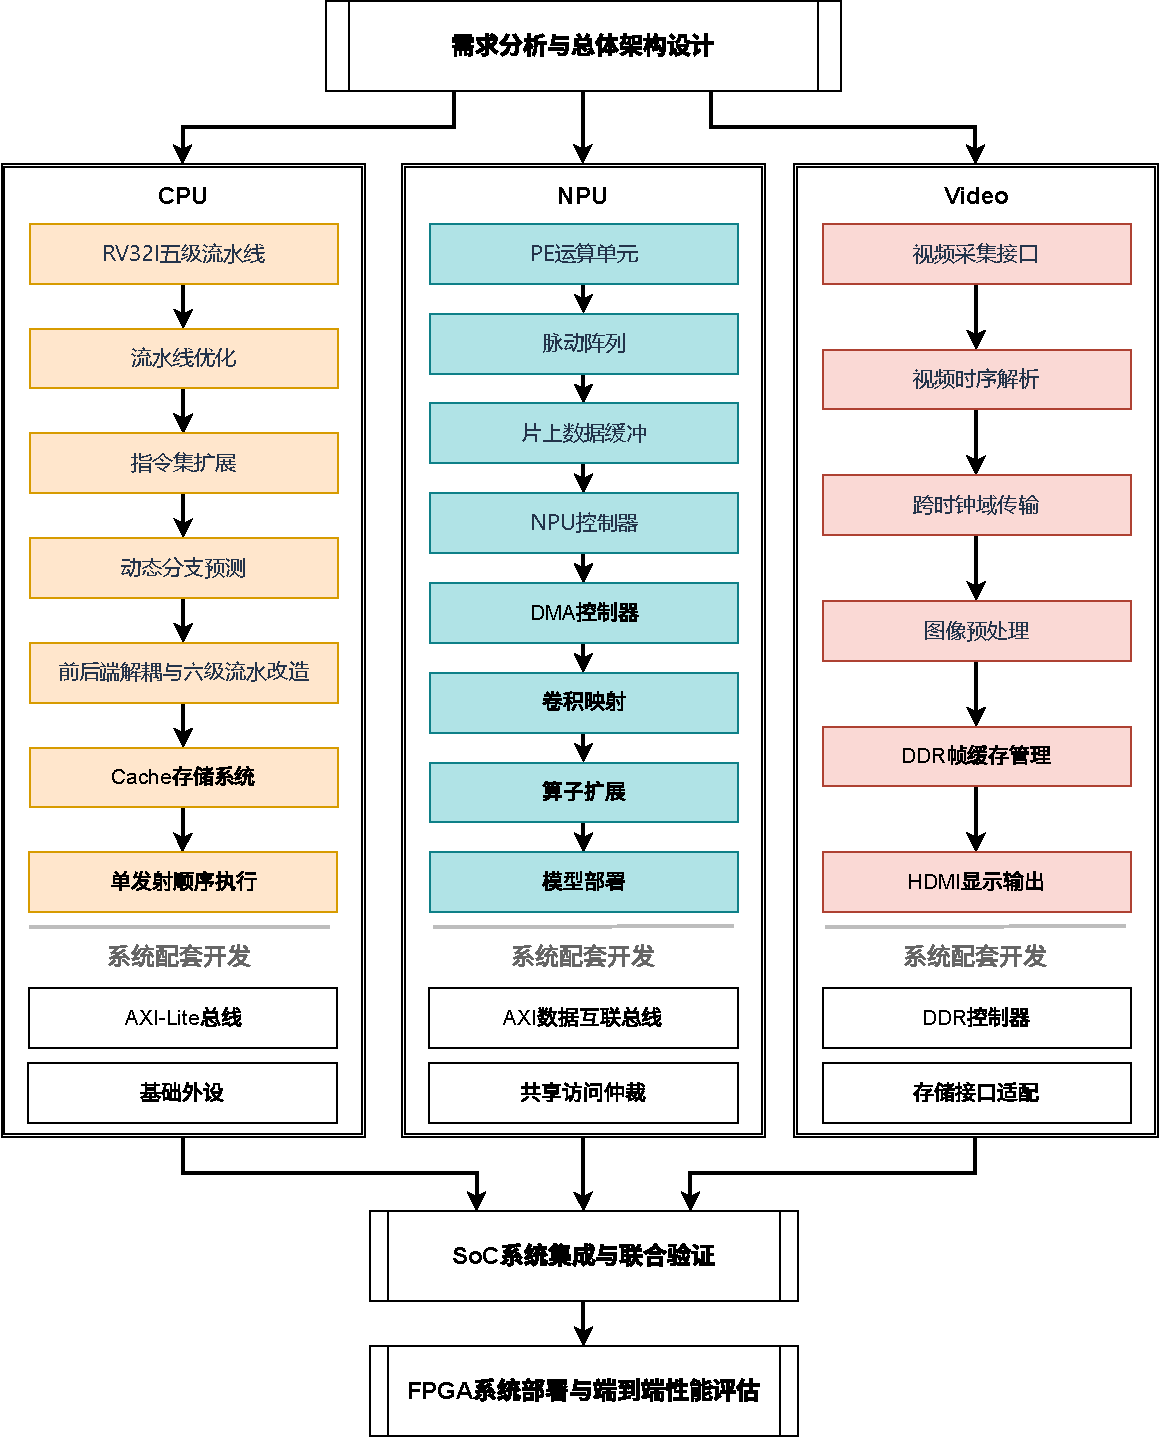
\includegraphics[width=\linewidth,height=0.78\textheight,keepaspectratio]{../figure/rv32-soc-page4.pdf}
\caption{TriHaRiscv设计流程}\label{fig:design-flow}
\end{figure}

\begin{enumerate}
    \item CPU路线完成六级单发射流水线、指令集、Cache、分支预测及异常中断设计，集成SoC互连与外设，
    实现定点检测后处理和帧调度。CoreMark、IPC及资源和时序分析贯穿各个可运行版本。
    \item NPU路线围绕固定YuNet计算图完成算子审计、量化和整数参考，设计PE、普通与深度卷积通路、片上缓冲及DMA，
    配套辅助算子和逐层数值核对，形成软件可调度的计算硬件与模型包。
    \item Video路线完成HDMI接收与发送、全帧采集、预览降采样及模型输入双线性缩放，设计三帧槽、输入格式化、显示行缓冲和头像叠加，
    通过显示记录提交、实际像素生效及旧帧释放确认连接软件调度和连续视频扫描。
\end{enumerate}

系统配套开发统一了DDR封装、AXI互连、时钟复位和公共配置。CPU负责互连和软件集成，Video负责DDR与像素域封装，
NPU提供计算接口、整数语义和模型数据。各路线通过CPU与NPU静态推理、CPU与Video控制、预处理与整数参考核对完成子系统联合验证。

FPGA部署将处理器、计算加速和视频链路集成到PG2L100H-6IFBG676，完成时钟、引脚和接口约束配置。
CPU性能采用CoreMark、CoreMark/MHz、CoreMark/LUT和IPC统计；FPGA实现分析最高工作频率（Fmax）与LUT、FF、DRM和APM资源占用。
应用端到端性能评估统计有效输出帧率、板内可见延迟、更新间隔及丢帧，结合逐层计算、DDR等待和CPU后处理定位开销。

\chapter{系统组成及功能说明}

\section{系统整体介绍}

\subsection{系统架构}

TriHaRiscv SoC采用CPU与NPU异构协同工作结构，系统架构如图\ref{fig:system-architecture}所示。
CPU执行控制程序和通用运算，NPU承担矩阵乘累加等计算任务。存储访问和外设配置通过不同的总线路径连接，
片上RAM、外部存储控制器和用户扩展接口构成系统的存储与输入输出部分。

\begin{center}
\begin{minipage}{\linewidth}
\centering
\captionsetup{type=figure,hypcap=false}
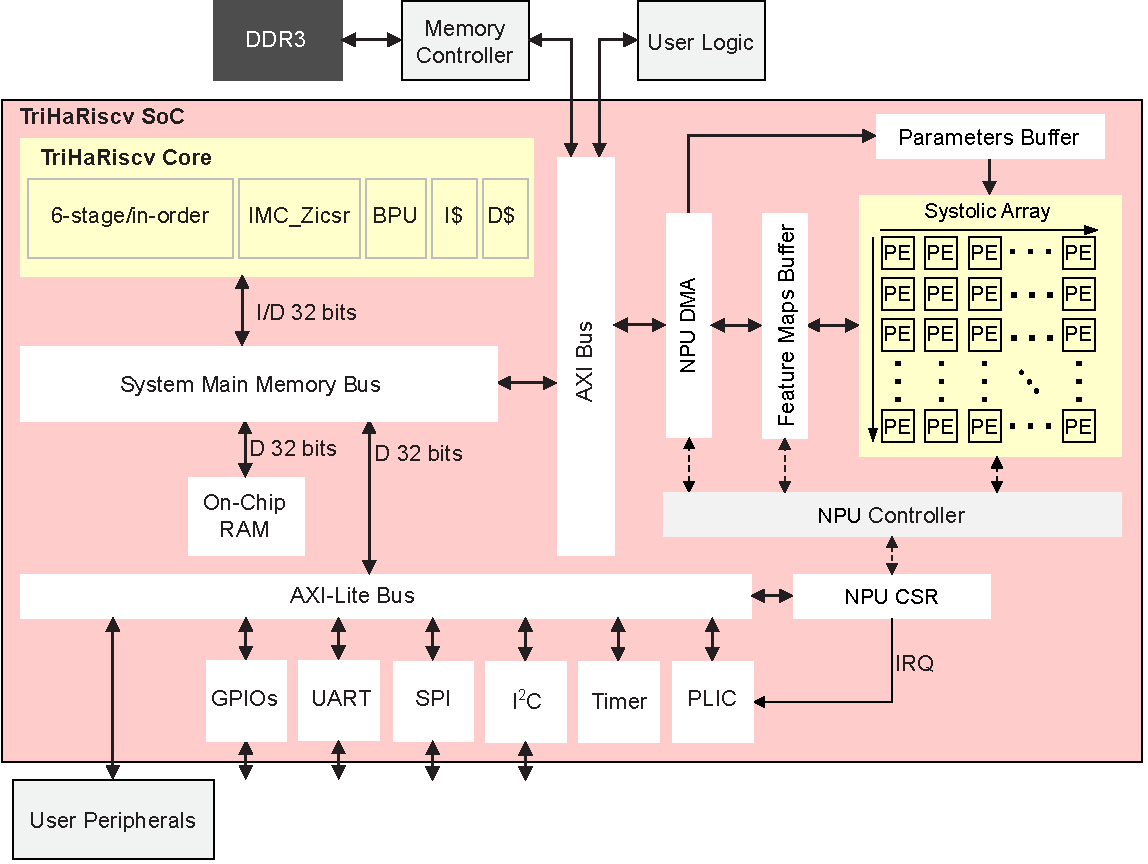
\includegraphics[width=\linewidth]{../figure/rv32-soc-page1.pdf}
\caption{TriHaRiscv SoC系统架构}\label{fig:system-architecture}
\end{minipage}
\end{center}

CPU采用六级双发射顺序执行结构，其指令和数据接口接入系统主存总线，连接片上RAM，
并经AXI通路访问外部存储。图中将DDR3及其存储控制器置于SoC边界之外，以区分处理
系统与板级存储接口。AXI-Lite通路用于访问外设寄存器和NPU控制寄存器，不承担NPU
的大批量数据搬运。

NPU包含控制器、DMA、特征图缓冲区、参数缓冲区和脉动阵列。CPU通过NPU控制寄存器
配置计算任务，DMA经AXI通路搬运特征图和参数，缓冲区为阵列提供计算数据。NPU控制
器协调数据传输和阵列运算，图中的中断通路用于返回任务完成通知。

SoC集成GPIO、UART、SPI、I\textsuperscript{2}C、定时器和PLIC等外设，各外设
通过AXI-Lite通路接入。PLIC汇聚NPU和外设的中断请求，并通知CPU处理。用户逻辑
和自定义外设分别通过相应的扩展接口接入系统。

\subsection{模块功能}

TriHaRiscv SoC划分为CPU、NPU、总线、存储、外设和视频六个模块，模块组成如图\ref{fig:soc-modules}所示。CPU和NPU分别封装为\texttt{triha\_cpu}和\texttt{triha\_npu}，其余模块提供系统互连、存储访问、外设控制及图像采集与显示功能。

\begin{center}
\begin{minipage}{\linewidth}
\centering
\captionsetup{type=figure,hypcap=false}
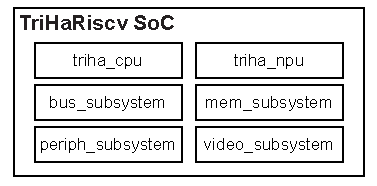
\includegraphics[width=0.5\linewidth]{../figure/rv32-soc-page2.pdf}
\caption{TriHaRiscv SoC模块图}\label{fig:soc-modules}
\end{minipage}
\end{center}

CPU通过\texttt{bus\_subsystem}访问存储空间和外设寄存器，并向NPU提交计算任务。
NPU通过DMA读取特征图和参数、写回计算结果；\texttt{mem\_subsystem}提供片上RAM
和外部存储的接入。\texttt{periph\_subsystem}集成通用外设及PLIC，将外设事件和
NPU任务完成中断送至CPU。

\texttt{video\_subsystem}完成像素接收、输入预处理、帧缓存管理和显示输出，CPU
负责视频链路配置、推理任务调度及显示结果发布。各模块的主要功能和接口见表\ref{tbl:module-roles}。

\begin{reporttable}
\begin{longtable}{@{}p{0.25\linewidth}p{0.41\linewidth}p{0.29\linewidth}@{}}
\caption{SoC模块功能表}\label{tbl:module-roles}\\
\toprule
模块 & 主要功能 & 主要接口 \\
\midrule
\endfirsthead
\caption[]{SoC模块功能表（续）}\\
\toprule
模块 & 主要功能 & 主要接口 \\
\midrule
\endhead
\bottomrule
\endfoot
\texttt{triha\_cpu} & 执行控制程序和通用运算，处理中断和异常 & 指令与数据访存接口、中断输入 \\
\texttt{triha\_npu} & 执行矩阵乘累加，调度DMA传输和阵列计算 & AXI数据接口、AXI-Lite寄存器接口、完成中断 \\
\texttt{bus\_subsystem} & 连接系统主从设备，完成地址译码、访问仲裁和协议桥接 & 主存总线、AXI与AXI-Lite接口 \\
\texttt{mem\_subsystem} & 提供片上RAM及外部存储接入，组织系统存储空间 & 片上RAM接口、外部存储访问接口 \\
\texttt{periph\_subsystem} & 集成GPIO、UART、SPI、I\textsuperscript{2}C、定时器和PLIC & AXI-Lite寄存器接口、外设信号与中断接口 \\
\texttt{video\_subsystem} & 完成图像采集、输入预处理、帧缓存管理和显示输出 & 视频输入输出接口、帧缓存读写接口 \\
\end{longtable}
\end{reporttable}

\section{CPU设计}

\subsection{CPU微架构}

{[}待填写{]}

\subsection{指令提取}

{[}待填写{]}

\subsection{指令译码}

{[}待填写{]}

\subsection{指令发射}

{[}待填写{]}

\subsection{指令执行}

{[}待填写{]}

\subsection{指令提交}

{[}待填写{]}

\subsection{存储管理}

{[}待填写{]}

\subsection{中断和异常}

{[}待填写{]}

\section{NPU设计}

\subsection{NPU微架构}

{[}待填写：总体框图、模块连接、支持的计算任务、CPU与NPU的协作关系，以及一次计算的执行流程。{]}

\subsection{PE计算单元}

{[}待填写：乘法器和累加器结构、输入与累加位宽、有符号运算、操作数传递，以及清零和使能控制。{]}

\subsection{脉动阵列}

{[}待填写：阵列规模、PE排列、边界接口、阵列互连、数据传播方向，以及结果读出方式。{]}

\subsection{阵列控制器}

{[}待填写：操作数锁存、波前注入、控制状态机、清零或续累加模式、计算时序、结束判定及完成握手。{]}

\subsection{DMA控制器}

{[}待填写：DDR数据搬入和结果写回、AXI突发传输、地址对齐、本地缓冲与预取、描述符队列、任务调度，以及背压和总线错误处理。{]}

\subsection{卷积展开单元}

{[}待填写：Im2Col实现、输入布局与寻址、卷积参数、边界补零、数据打包、硬件支持范围，以及功能关闭时的软件回退。{]}

\subsection{定点后处理单元}

{[}待填写：仿射变换、移位缩放、舍入规则、INT8饱和、零点与激活处理，以及硬件功能开关和软件分工。{]}

\subsection{寄存器接口}

{[}待填写：MMIO寄存器映射、字段定义、读写属性、软件配置和启动顺序、状态查询、状态清除，以及中断通知机制。{]}

\section{系统互连与存储}

\subsection{总线结构}

{[}待填写：控制总线和数据总线、主从设备连接、访问宽度，以及必要的协议桥接和跨时钟域路径。{]}

\subsection{存储组织}

{[}待填写：片上RAM和DDR的容量与组织、地址映射、缓存别名、模型参数和运行工作区分配、字节序，以及各区域的用途和访问限制。{]}

\begin{reporttable}
\begin{longtable}{@{}p{0.23\linewidth}p{0.34\linewidth}p{0.35\linewidth}@{}}
\caption{系统地址映射表}\\
\toprule
区域 & 实际地址 & 用途与访问限制 \\
\midrule
\endfirsthead
\caption[]{系统地址映射表（续）}\\
\toprule
区域 & 实际地址 & 用途与访问限制 \\
\midrule
\endhead
\bottomrule
\endfoot
{[}待填写{]} & {[}待填写{]} & {[}待填写{]} \\
{[}待填写{]} & {[}待填写{]} & {[}待填写{]} \\
{[}待填写{]} & {[}待填写{]} & {[}待填写{]} \\
{[}待填写{]} & {[}待填写{]} & {[}待填写{]} \\
\end{longtable}
\end{reporttable}

\subsection{访问仲裁}

{[}待填写：CPU、NPU和视频链路的并发请求、仲裁策略、事务归属、占用与释放条件，以及背压处理。{]}

\subsection{共享数据访问约定}

{[}待填写：缓存与DMA的数据可见性、共享缓冲区访问权限、数据同步顺序、缓存维护要求、软件维护责任，以及一致性约定。{]}

\section{图像采集与显示链路}

\subsection{图像采集}

{[}待填写：传感器初始化、DVP接口、像素接收、有效帧判据、输入像素格式、写入完整性，以及采集错误处理。{]}

\subsection{输入预处理}

{[}待填写：图像裁剪、像素格式转换、数据打包、模型输入生成，以及软硬件分工。{]}

\subsection{帧缓存管理}

{[}待填写：帧缓存容量和布局、帧标识、任务及模型标识、采集/推理/显示的缓冲区所有权转移、结果发布原子性、丢帧策略，以及复位和错误恢复。{]}

\subsection{显示输出}

{[}待填写：帧数据读取、扫描时序、原图与结果的同帧配对、显示接口配置，以及像素输出格式。{]}

\section{模型部署}

\subsection{模型选型}

{[}待填写：模型来源、许可证、网络结构、输入输出规格、输入尺寸和颜色顺序，以及选择依据。{]}

\subsection{量化方案}

{[}待填写：权重和激活的数据类型、量化参数、累加位宽、混合精度处理、舍入和溢出约定，以及数值参考。{]}

\subsection{模型导出}

{[}待填写：计算图描述、参数文件、张量布局、模型元数据、版本和哈希标识、部署文件生成方式，以及完整性检查。{]}

\subsection{算子映射}

{[}待填写：各算子及执行阶段的CPU/NPU分工、硬件支持范围、分块执行、软件回退条件，以及数值参考和限制。{]}

\begin{reporttable}
\begin{longtable}{@{}p{0.18\linewidth}p{0.24\linewidth}p{0.22\linewidth}p{0.30\linewidth}@{}}
\caption{算子执行方式表}\\
\toprule
算子或阶段 & 执行后端 & 实际支持范围 & 数值参考与限制 \\
\midrule
\endfirsthead
\caption[]{算子执行方式表（续）}\\
\toprule
算子或阶段 & 执行后端 & 实际支持范围 & 数值参考与限制 \\
\midrule
\endhead
\bottomrule
\endfoot
{[}待填写{]} & {[}待填写{]} & {[}待填写{]} & {[}待填写{]} \\
{[}待填写{]} & {[}待填写{]} & {[}待填写{]} & {[}待填写{]} \\
{[}待填写{]} & {[}待填写{]} & {[}待填写{]} & {[}待填写{]} \\
{[}待填写{]} & {[}待填写{]} & {[}待填写{]} & {[}待填写{]} \\
\end{longtable}
\end{reporttable}

\subsection{裸机运行时}

{[}待填写：软件层次、启动初始化、链接布局、模型加载、MMIO驱动调用、固定工作区、张量缓冲复用、资源生命周期、日志和错误返回。{]}

\subsection{推理流程}

{[}待填写：软件入口、输入准备、调用链、逐层调度、任务提交和完成检查、后处理、结果交付、失败回退，以及输入输出接口。{]}

\section{FPGA实现}

FPGA顶层集成了SoC、时钟复位模块，以及存储和板级接口封装，模块组成如图\ref{fig:fpga-top-modules}所示。\texttt{triha\_soc}封装图\ref{fig:soc-modules}中的六个SoC模块，顶层通过各接口封装连接外部存储、摄像头、显示设备和通用外设。

\begin{center}
\begin{minipage}{\linewidth}
\centering
\captionsetup{type=figure,hypcap=false}
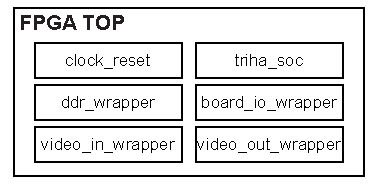
\includegraphics[width=0.5\linewidth]{../figure/rv32-soc-page3.pdf}
\caption{FPGA顶层模块图}\label{fig:fpga-top-modules}
\end{minipage}
\end{center}

\texttt{clock\_reset}根据板级参考时钟生成各时钟域的工作时钟，并按初始化顺序生成与释放复位信号。\texttt{ddr\_wrapper}封装DDR3控制器和厂商存储接口，为CPU、NPU及视频帧缓存提供外部存储访问通路。\texttt{board\_io\_wrapper}连接UART、GPIO、SPI和I\textsuperscript{2}C等板级信号，完成SoC内部接口与FPGA引脚之间的适配。

\texttt{video\_in\_wrapper}接入摄像头像素及帧、行同步信号，将其送入SoC视频子系统；\texttt{video\_out\_wrapper}接收视频子系统输出的像素和同步信号，连接板级显示接口。厂商IP及板级信号适配集中在顶层封装模块中，SoC内部保留处理、互连和视频链路的功能逻辑。

\subsection{目标平台}

本设计采用盘古100pro+开发板作为验证平台，主控为紫光同创Logos-2系列FPGA，器件型号为 PG2L100H-6IFBG676。CPU、NPU、系统互连和视频处理逻辑部署在该器件中，利用片上逻辑、APM运算单元和DRM存储块完成计算与数据缓冲。
板载DDR3由两颗4Gbit芯片组成，总容量为1GB，通过32bit数据通路连接FPGA，用于存放模型参数、特征图和视频帧。HDMI输入输出接口连接视频链路，USB-UART接口承担裸机程序的串口通信和调试。平台主要配置见表\ref{tbl:platform}。

\begin{reporttable}
\footnotesize
\begin{longtable}{@{}lll@{}}
\caption{平台配置表}\label{tbl:platform}\\
\toprule
项目 & 配置 & 说明或用途 \\
\midrule
\endfirsthead
\caption[]{平台配置表（续）}\\
\toprule
项目 & 配置 & 说明或用途 \\
\midrule
\endhead
\bottomrule
\endfoot
开发板 & 盘古100pro+（MES2L676-100HP） & FPGA及板级外设平台 \\
主控器件 & PG2L100H-6IFBG676 & 紫光同创Logos-2系列FPGA \\
逻辑资源 & 66,600个LUT，133,200个FF & CPU、NPU及系统控制逻辑 \\
运算资源 & 240个APM & 乘法与MAC运算 \\
片上存储 & 155个36Kbit DRM & CPU存储、Cache及NPU缓冲区 \\
外部存储 & 1GB DDR3，2颗4Gbit芯片，32bit数据位宽 & 模型参数、特征图及视频帧存储 \\
视频接口 & 1路HDMI输入、1路HDMI输出 & 视频接入与显示 \\
通信接口 & USB-UART & 板载通信与串口调试 \\
辅助接口 & 按键、LED、SD卡接口 & 控制输入、状态显示及扩展存储 \\
下载与供电 & JTAG、12V电源接口 & 比特流下载、逻辑调试和板卡供电 \\
\end{longtable}
\end{reporttable}

\subsection{工程配置}

{[}待填写：工具版本、顶层模块、源码组织、功能开关、厂商IP和官方例程的引用版本及修改范围，以及综合、布局布线和位流生成流程。{]}

\subsection{时钟复位}

{[}待填写：时钟来源、频率与PLL配置、时钟域划分、复位顺序、DDR初始化依赖以及跨域处理的总体安排。{]}

\subsection{板级接口}

{[}待填写：摄像头、显示、DDR和UART等板级接口的引脚映射、信号方向、I/O标准、电平要求、连接关系及接口配置。{]}

\subsection{实现约束}

{[}待填写：时钟约束、输入输出时序约束、跨域约束、时序例外及其依据、尚未确认的外部接口条件，以及约束覆盖范围和待闭合事项。{]}

\chapter{完成情况及性能参数}

\section{整体介绍}

{[}待填写：工程版本与源码提交、目标平台与器件、运行配置、工具版本、整体完成情况，以及仿真验证、FPGA实现和实物验证的范围与边界。{]}

\section{工程成果}

\subsection{硬件成果}

{[}待填写：CPU、NPU、系统互连、存储及图像采集与显示链路的实现成果，FPGA集成情况，以及对应RTL、板级工程、约束文件和硬件交付清单。{]}

\subsection{软件成果}

{[}待填写：模型导出与量化部署、裸机运行时、外设和NPU驱动、CPU回退路径、运行程序及配套工具的实现成果，以及软件交付清单和复现入口。{]}

\subsection{功能验证}

{[}待填写：CPU指令执行、NPU计算、数据搬运、共享存储访问、图像链路和完整模型运行的验证结论，已通过项目、待验证项目与已知限制，以及对应附录中的测试用例、波形和日志索引。{]}

\subsection{应用演示}

{[}待填写：系统连接与板卡接口、启动和操作流程、输入输出图像、连续帧运行效果及演示条件；分别标明仿真演示与实物演示，并列出实物照片、传感器、显示输出和运行画面的实际验证状态。{]}

\section{特性成果}

\subsection{CPU性能}

{[}待填写：测试程序、编译选项与运行配置、执行周期、退休指令数、IPC及相关性能计数器，统计口径、测试结果和影响因素；区分仿真结果与板上实测结果，注明基准测试的运行条件和结果适用范围。{]}

\subsection{NPU性能}

{[}待填写：测试算子与矩阵规模、计算周期、DMA数据搬运开销、阵列利用率，以及相同任务和数值约定下相对CPU执行的加速比；说明计时范围、运行配置和测量方法，区分计算单元性能与包含搬运的任务性能。{]}

\subsection{系统性能}

{[}待填写：模型与输入尺寸、完整模型推理延迟、端到端处理延迟、连续帧吞吐率、CPU与NPU协同执行开销，以及系统瓶颈分析；说明各项指标的计时起止点、测试条件和证据类型，区分仿真推算与板上实测。{]}

\subsection{FPGA实现指标}

{[}待填写：目标器件与工程配置、逻辑资源、寄存器、DSP和存储资源占用，工作频率、时序裕量及关键路径；注明报告来自综合还是布局布线阶段，并区分时序约束目标、实现结果和实际板上工作条件。{]}

% !TEX root = ../技术文档.tex
\chapter{总\ \ 结}

% !TEX root = ../../技术文档.tex
\section{可扩展之处}

系统以主人脸矩形定位并缩放固定透明头像，可进一步接入关键点或表情模型，扩展对齐方式和素材选择。
扩展时在现有帧调度中增加裁脸、缩放和分类阶段，将结果写入公共显示记录，并配置相应的像素合成通路。
多素材应用可沿用头像编号与代次管理，分别生成素材布局及校验信息；素材切换与同帧原图保持一致。
新增模型、素材访问和后处理开销应计入整机帧率、延迟及片上存储预算。

CPU可进一步研究前端供数、预测策略和流水线并行度，NPU可扩展算子及并行规模。
扩展工作沿用公共地址、寄存器和版本管理方式，分别检查指令语义、整数结果、共享存储顺序及FPGA时序资源。


% !TEX root = ../../技术文档.tex
\section{心得体会}

本次参赛，我们以自主设计 RISC-V 处理器为核心，希望不仅完成 CPU 的功能验证和性能测试，还能将其部署到国产 FPGA 上，通过实际视觉应用检验处理器与硬件加速器的协同工作能力。在研发过程中，我们逐渐认识到，单个模块的性能固然重要，但如何在有限的硬件资源下完成系统集成，并保证各模块稳定运行，同样是 FPGA 设计中不可忽视的挑战。

CPU设计是本次作品投入精力最多的部分。我们从已有的五级流水线出发，逐步完成六级流水线、动态分支预测、Cache 和可配置双发射结构的设计。双发射的实现尤其让我们体会到处理器设计的复杂性：增加第二条执行通路只是其中一步，还必须解决指令配对、数据相关、结果前递、共享运算资源和异常恢复等问题。为了保证执行正确性，我们针对分支恢复、访存等待和错误路径副作用设计了定向测试。在一次零比较分支配对测试中，我们还发现测试平台自身的输入条件与现有设计不一致。这让我们认识到，验证不仅是检查设计能否通过测试，还需要保证测试条件与硬件实际行为相符。

NPU 与视频系统的集成使我们对软硬件协同设计有了更加具体的理解。 NPU 的设计需要从 YuNet 的实际算子和数据规模出发，在计算并行度、片上缓冲容量和数据搬运开销之间作出取舍。视频链路则不仅需要完成采集和图像叠加，还必须确保检测结果与原始画面对应。为此，我们设计了三帧槽管理和显示释放确认机制，并通过流式合成实现检测框及透明头像叠加。在头像功能中，利用无损行区间缓存减少片上纹理存储占用，也使我们更加直观地认识到，针对具体应用特点优化存储组织，往往比单纯增加硬件资源更有效。

在 FPGA 上板过程中，我们进一步体会到，仿真正确并不意味着系统集成就已经完成。时钟域交互、DDR 访问、存储器响应以及布局布线后的时序约束，都可能成为影响系统运行的关键因素。因此，我们采用模块验证、系统联合仿真与板级测试相结合的方式，逐步排查问题，并通过统一接口和配置管理减少不同模块集成时的差异。

目前，作品已经实现完整的人脸检测与头像叠加板级演示，但整网推理速度仍有较大的优化空间。这也让我们认识到，硬件设计不能只关注理论计算峰值，还应当结合实际执行周期，分析数据搬运、控制调度及计算单元的利用情况。

通过本次比赛，我们不仅加深了对 RISC-V 处理器微架构和 FPGA 硬件设计的理解，也积累了从 RTL 开发、功能验证到系统集成和实板调试的工程经验。相比单独完成某个模块，能够让自主设计的 CPU、NPU 和视频系统共同运行，并通过真实应用检验设计，是本次参赛最有价值的收获。


\chapter{参考文献}

% 在 reference/project.bib 添加实际引用后，在此加入 BibTeX 编译命令。

\ifreportdraft
  \chapter*{附\ \ 录}
\addcontentsline{toc}{chapter}{附\ \ 录}

\setcounter{section}{0}
\renewcommand{\thesection}{\Alph{section}}
\renewcommand{\theHsection}{appendix.\Alph{section}}
\renewcommand{\theHsubsection}{\theHsection.\arabic{subsection}}
\counterwithin{figure}{section}
\counterwithin{table}{section}
\counterwithin{equation}{section}
\renewcommand{\thefigure}{\thesection-\arabic{figure}}
\renewcommand{\thetable}{\thesection-\arabic{table}}
\renewcommand{\theequation}{\thesection-\arabic{equation}}
\renewcommand{\theHfigure}{\theHsection.\arabic{figure}}
\renewcommand{\theHtable}{\theHsection.\arabic{table}}
\renewcommand{\theHequation}{\theHsection.\arabic{equation}}

\section{仿真环境与验证方法}

\subsection{工具配置}

{[}待填写：仿真器、RISC-V编译工具、参考模型及依赖工具的版本，源码提交、配置参数、运行命令和日志保存位置。{]}

\subsection{测试平台}

{[}待填写：单元、模块和系统级测试的划分，测试台结构、时钟复位、输入生成方式及输出采集方式；说明仿真覆盖范围，不将仿真结果视为板级电气或实物验证结论。{]}

\subsection{判定标准}

{[}待填写：各类测试的验证目的、参考模型、期望行为、数值误差容限、超时条件和通过标准，以及波形、数值结果和验证结论的记录方式。{]}

\section{CPU仿真验证}

\subsection{指令集验证}

{[}待填写：支持的RV32指令集能力与扩展配置、官方架构测试及定向用例，未启用扩展的非法指令行为、测试结果和已知限制。{]}

\subsection{流水线控制}

{[}待填写：译码、发射和提交行为，数据冒险、旁路、暂停和冲刷的验证用例，关键流水线信号、退休结果及判定依据。{]}

\subsection{指令提取}

{[}待填写：取指时序、压缩指令处理、分支预测和重定向的测试输入与关键波形；验证压缩指令配置下预测查询、更新及相关性能计数器的行为。{]}

\subsection{指令执行}

{[}待填写：整数运算、移位、比较和乘除法的测试配置，符号组合、边界输入及除法特殊情况，与参考结果的逐项比较和执行完成时序。{]}

\subsection{中断和异常}

{[}待填写：已实现CSR的读写行为、异常触发、中断响应和返回流程，异常原因与返回地址、流水线处理及关键波形的判定结果。{]}

\subsection{存储访问}

{[}待填写：缓存命中与未命中、读写访问、字节使能、访问对齐和PMA边界的验证用例，访存时序、读回数据及异常行为。{]}

\section{NPU仿真验证}

\subsection{计算正确性}

{[}待填写：PE和脉动阵列的测试输入、INT8乘法与INT32累加约定，符号组合、累加边界、参考结果及逐项数值比较。{]}

\subsection{分块计算}

{[}待填写：矩阵规模、数据布局、分块参数和尾块处理的测试组合，输入输出地址、块间拼接及与完整矩阵参考计算的比较结果。{]}

\subsection{DMA传输}

{[}待填写：DMA读写搬运、传输长度、地址边界、突发传输和背压场景，握手波形、内存读回数据及传输完成结果。{]}

\subsection{任务控制}

{[}待填写：寄存器配置、任务启动、忙闲状态、完成通知和连续任务提交的测试序列，以及异常输入、背压和任务重新启动时的状态转换。{]}

\subsection{可选功能}

{[}待填写：卷积展开、定点后处理等已实现可选功能的测试输入、参考结果和边界情况；分别记录开启与关闭配置下的功能行为、合法响应及回退路径。{]}

\section{系统互连与存储仿真验证}

\subsection{总线协议}

{[}待填写：总线各通道握手、突发传输、字节使能和响应行为的测试配置，背压场景、关键协议波形及通过标准。{]}

\subsection{访问仲裁}

{[}待填写：多主设备并发访问、持续请求和不同背压条件下的测试序列，仲裁顺序、请求完成情况及背压传播结果。{]}

\subsection{地址译码}

{[}待填写：地址映射、存储与外设访问边界、非法地址及禁用模块访问的测试用例，目标选择、读写结果和错误响应。{]}

\subsection{共享数据访问}

{[}待填写：CPU、NPU DMA和图像链路的共享数据访问场景，缓冲区交接、缓存维护、数据可见性及读写结果的验证；按实际访问约定检查，不假定硬件自动维持缓存一致性。{]}

\section{图像采集与显示链路仿真验证}

\subsection{图像采集}

{[}待填写：图像输入时序、帧同步、行同步、像素有效信号、像素格式和帧标识的测试配置，采集数据及帧完整性的判定结果。{]}

\subsection{输入预处理}

{[}待填写：已实现的像素格式转换、尺寸处理和模型输入组织，测试图像、输入输出尺寸、通道排列及与参考处理结果的比较。{]}

\subsection{跨时钟域}

{[}待填写：不同采集、处理和显示时钟条件下的跨域同步，数据与控制信号传递、复位恢复及边界时序的测试波形和判定结果。{]}

\subsection{帧缓存}

{[}待填写：帧缓存读写、缓冲区切换、所有权交接和读写冲突的测试场景，帧完整性、数据保持及冲突处理结果。{]}

\subsection{显示输出}

{[}待填写：显示扫描、像素输出、同帧结果配对和输入输出一致性的仿真配置，输出时序、参考像素及显示数据核对结果。{]}

\section{系统联合仿真验证}

\subsection{完整模型推理}

{[}待填写：模型版本、输入尺寸、算子执行后端及测试输入，CPU与NPU协同、端到端数据流和推理完成情况，运行日志及验证边界。{]}

\subsection{连续帧处理}

{[}待填写：多帧输入顺序、帧标识、任务衔接和缓冲区交接的测试序列，连续运行中的完成通知、帧配对及结果保持情况。{]}

\subsection{运行配置}

{[}待填写：加速启用与禁用、CPU回退及显示配置组合的测试矩阵，各配置的运行路径、任务完成情况和结果一致性；区别于单个NPU可选功能的验证。{]}

\subsection{结果核对}

{[}待填写：整网输出与软件参考结果的比较、数值误差统计、帧标识及结果配对检查，参考图像、核对日志和通过结论；注明误差容限与未覆盖项目。{]}

\else
  \ifreleaseappendix
    \chapter*{附\ \ 录}
\addcontentsline{toc}{chapter}{附\ \ 录}

\setcounter{section}{0}
\renewcommand{\thesection}{\Alph{section}}
\renewcommand{\theHsection}{appendix.\Alph{section}}
\renewcommand{\theHsubsection}{\theHsection.\arabic{subsection}}
\counterwithin{figure}{section}
\counterwithin{table}{section}
\counterwithin{equation}{section}
\renewcommand{\thefigure}{\thesection-\arabic{figure}}
\renewcommand{\thetable}{\thesection-\arabic{table}}
\renewcommand{\theequation}{\thesection-\arabic{equation}}
\renewcommand{\theHfigure}{\theHsection.\arabic{figure}}
\renewcommand{\theHtable}{\theHsection.\arabic{table}}
\renewcommand{\theHequation}{\theHsection.\arabic{equation}}

\section{仿真环境与验证方法}

\subsection{工具配置}

{[}待填写：仿真器、RISC-V编译工具、参考模型及依赖工具的版本，源码提交、配置参数、运行命令和日志保存位置。{]}

\subsection{测试平台}

{[}待填写：单元、模块和系统级测试的划分，测试台结构、时钟复位、输入生成方式及输出采集方式；说明仿真覆盖范围，不将仿真结果视为板级电气或实物验证结论。{]}

\subsection{判定标准}

{[}待填写：各类测试的验证目的、参考模型、期望行为、数值误差容限、超时条件和通过标准，以及波形、数值结果和验证结论的记录方式。{]}

\section{CPU仿真验证}

\subsection{指令集验证}

{[}待填写：支持的RV32指令集能力与扩展配置、官方架构测试及定向用例，未启用扩展的非法指令行为、测试结果和已知限制。{]}

\subsection{流水线控制}

{[}待填写：译码、发射和提交行为，数据冒险、旁路、暂停和冲刷的验证用例，关键流水线信号、退休结果及判定依据。{]}

\subsection{指令提取}

{[}待填写：取指时序、压缩指令处理、分支预测和重定向的测试输入与关键波形；验证压缩指令配置下预测查询、更新及相关性能计数器的行为。{]}

\subsection{指令执行}

{[}待填写：整数运算、移位、比较和乘除法的测试配置，符号组合、边界输入及除法特殊情况，与参考结果的逐项比较和执行完成时序。{]}

\subsection{中断和异常}

{[}待填写：已实现CSR的读写行为、异常触发、中断响应和返回流程，异常原因与返回地址、流水线处理及关键波形的判定结果。{]}

\subsection{存储访问}

{[}待填写：缓存命中与未命中、读写访问、字节使能、访问对齐和PMA边界的验证用例，访存时序、读回数据及异常行为。{]}

\section{NPU仿真验证}

\subsection{计算正确性}

{[}待填写：PE和脉动阵列的测试输入、INT8乘法与INT32累加约定，符号组合、累加边界、参考结果及逐项数值比较。{]}

\subsection{分块计算}

{[}待填写：矩阵规模、数据布局、分块参数和尾块处理的测试组合，输入输出地址、块间拼接及与完整矩阵参考计算的比较结果。{]}

\subsection{DMA传输}

{[}待填写：DMA读写搬运、传输长度、地址边界、突发传输和背压场景，握手波形、内存读回数据及传输完成结果。{]}

\subsection{任务控制}

{[}待填写：寄存器配置、任务启动、忙闲状态、完成通知和连续任务提交的测试序列，以及异常输入、背压和任务重新启动时的状态转换。{]}

\subsection{可选功能}

{[}待填写：卷积展开、定点后处理等已实现可选功能的测试输入、参考结果和边界情况；分别记录开启与关闭配置下的功能行为、合法响应及回退路径。{]}

\section{系统互连与存储仿真验证}

\subsection{总线协议}

{[}待填写：总线各通道握手、突发传输、字节使能和响应行为的测试配置，背压场景、关键协议波形及通过标准。{]}

\subsection{访问仲裁}

{[}待填写：多主设备并发访问、持续请求和不同背压条件下的测试序列，仲裁顺序、请求完成情况及背压传播结果。{]}

\subsection{地址译码}

{[}待填写：地址映射、存储与外设访问边界、非法地址及禁用模块访问的测试用例，目标选择、读写结果和错误响应。{]}

\subsection{共享数据访问}

{[}待填写：CPU、NPU DMA和图像链路的共享数据访问场景，缓冲区交接、缓存维护、数据可见性及读写结果的验证；按实际访问约定检查，不假定硬件自动维持缓存一致性。{]}

\section{图像采集与显示链路仿真验证}

\subsection{图像采集}

{[}待填写：图像输入时序、帧同步、行同步、像素有效信号、像素格式和帧标识的测试配置，采集数据及帧完整性的判定结果。{]}

\subsection{输入预处理}

{[}待填写：已实现的像素格式转换、尺寸处理和模型输入组织，测试图像、输入输出尺寸、通道排列及与参考处理结果的比较。{]}

\subsection{跨时钟域}

{[}待填写：不同采集、处理和显示时钟条件下的跨域同步，数据与控制信号传递、复位恢复及边界时序的测试波形和判定结果。{]}

\subsection{帧缓存}

{[}待填写：帧缓存读写、缓冲区切换、所有权交接和读写冲突的测试场景，帧完整性、数据保持及冲突处理结果。{]}

\subsection{显示输出}

{[}待填写：显示扫描、像素输出、同帧结果配对和输入输出一致性的仿真配置，输出时序、参考像素及显示数据核对结果。{]}

\section{系统联合仿真验证}

\subsection{完整模型推理}

{[}待填写：模型版本、输入尺寸、算子执行后端及测试输入，CPU与NPU协同、端到端数据流和推理完成情况，运行日志及验证边界。{]}

\subsection{连续帧处理}

{[}待填写：多帧输入顺序、帧标识、任务衔接和缓冲区交接的测试序列，连续运行中的完成通知、帧配对及结果保持情况。{]}

\subsection{运行配置}

{[}待填写：加速启用与禁用、CPU回退及显示配置组合的测试矩阵，各配置的运行路径、任务完成情况和结果一致性；区别于单个NPU可选功能的验证。{]}

\subsection{结果核对}

{[}待填写：整网输出与软件参考结果的比较、数值误差统计、帧标识及结果配对检查，参考图像、核对日志和通过结论；注明误差容限与未覆盖项目。{]}

  \fi
\fi
\end{document}
